%% \chapter[htoc-titlei][hhead-titlei]{htitlei}
%% -----------------------------------------------------------------------------
\chapter[Analysis Summary][Analysis Summary]{Analysis Summary}
\label{chapter:analysis} 
OVERLAP REMOVAL

This chapter provides an overview the of analysis searching for SM
production of the Higgs boson in association with top quarks in
multi-lepton final states. The analysis searches in signal regions
with 2 same-sign, 3 and 4 light leptons ($e, \mu$), which are sensitive to Higgs
decays to vector bosons, $H\rightarrow W^{\pm}W^{\pm}$ and $H\rightarrow
Z^{\pm}Z^{\pm}$. It forms a complement to already completed searches for in
final states targeting the $H\rightarrow b\bar{b}$ \cite{Aad:2014lma},
$H\rightarrow\gamma\gamma$\cite{ATLAS-CONF-2014-011}. The \tth searches
in the $H\rightarrow\tau\tau$ decay modes were developed concurrently with teh 
multi-lepton searches, but we do not discuss these there. 
Of these complementary searches, the multi-lepton and $bb$ channels are the most sensitve. 

Based on SM production cross-sections, observation lies just outside the sensitivity
of the Run I dataset, even when combining all searches. Intead, the analyses provide an opportunity to 
constrain for the first time the \tth production mode with limits reasonably close to the
actual production rate. The multi-lepton analysis is optimized to overall sensitivity to the 
\tth production rather than individual decay modes, which would be more useful for
constraining Higgs couplings. 

Detailed description of the event and objection section are provided in Chapter \ref{chapter:selection},
background modeling in Chapter \ref{chapter:background}, the effect of systematic errors and the 
statistical analysis in Chapter \ref{chapter:systematics} and final results in Chapter \ref{chapter:results}.


\section{Signal Characteristics} 

\begin{figure}[!t]
\centering
\begin{tabular}{ccc}
\subfloat[2$\ell$ SS]{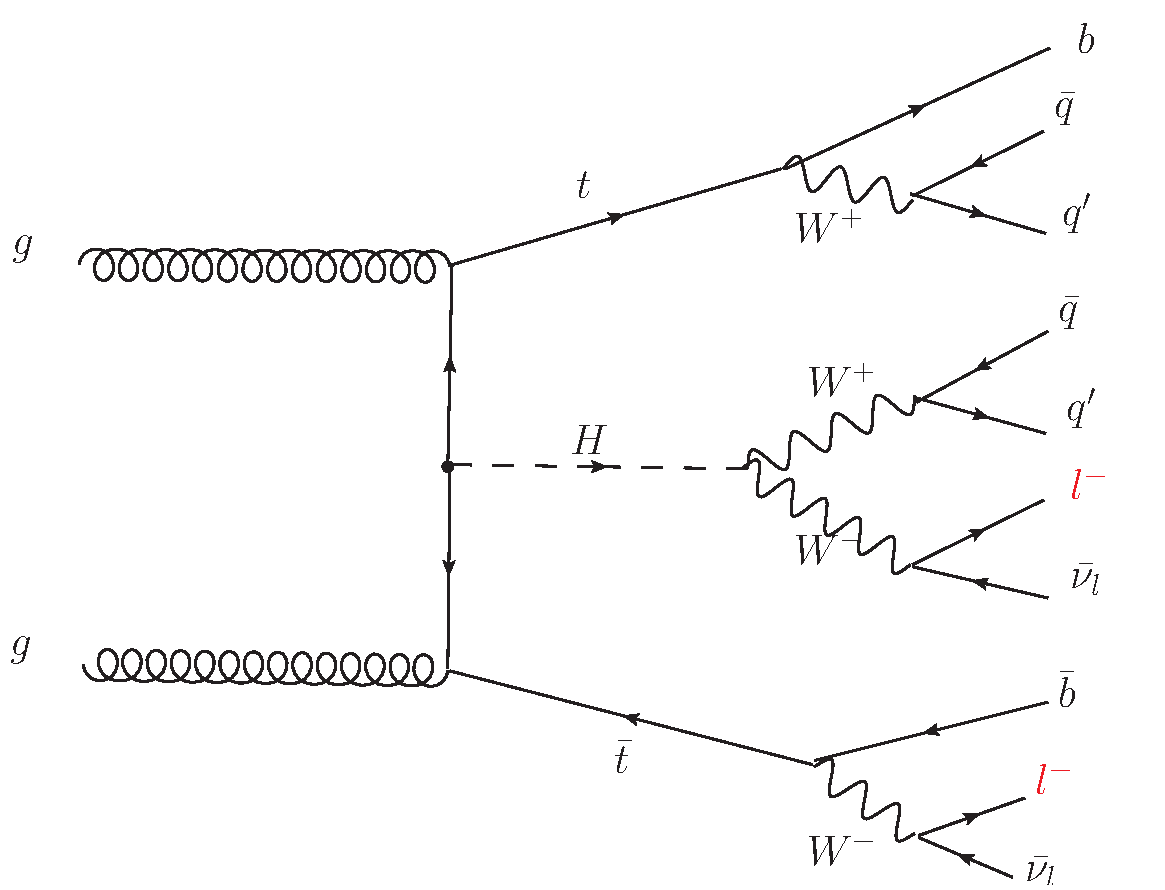
\includegraphics[width=0.30\textwidth]{figs/analysis/2l.pdf}} &
\subfloat[3$\ell$]{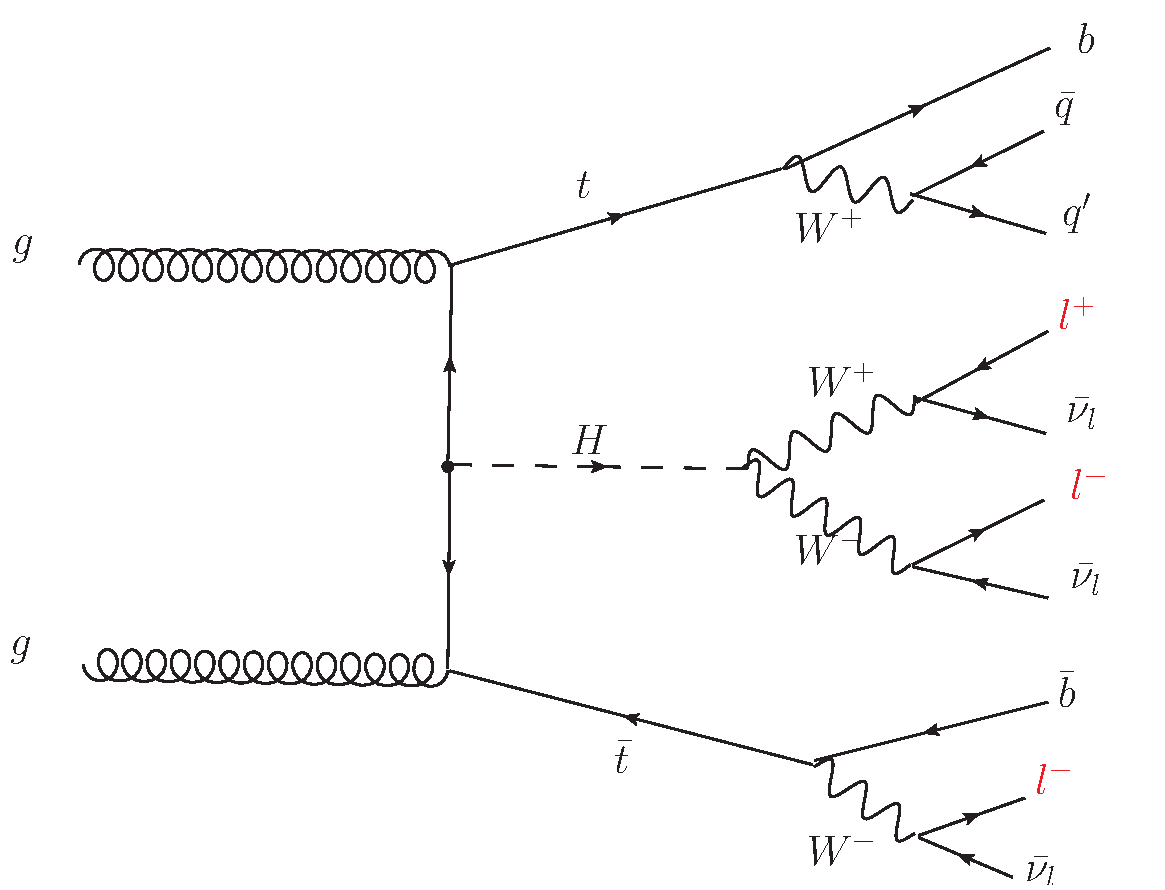
\includegraphics[width=0.30\textwidth]{figs/analysis/3l.pdf}} &
\subfloat[4$\ell$]{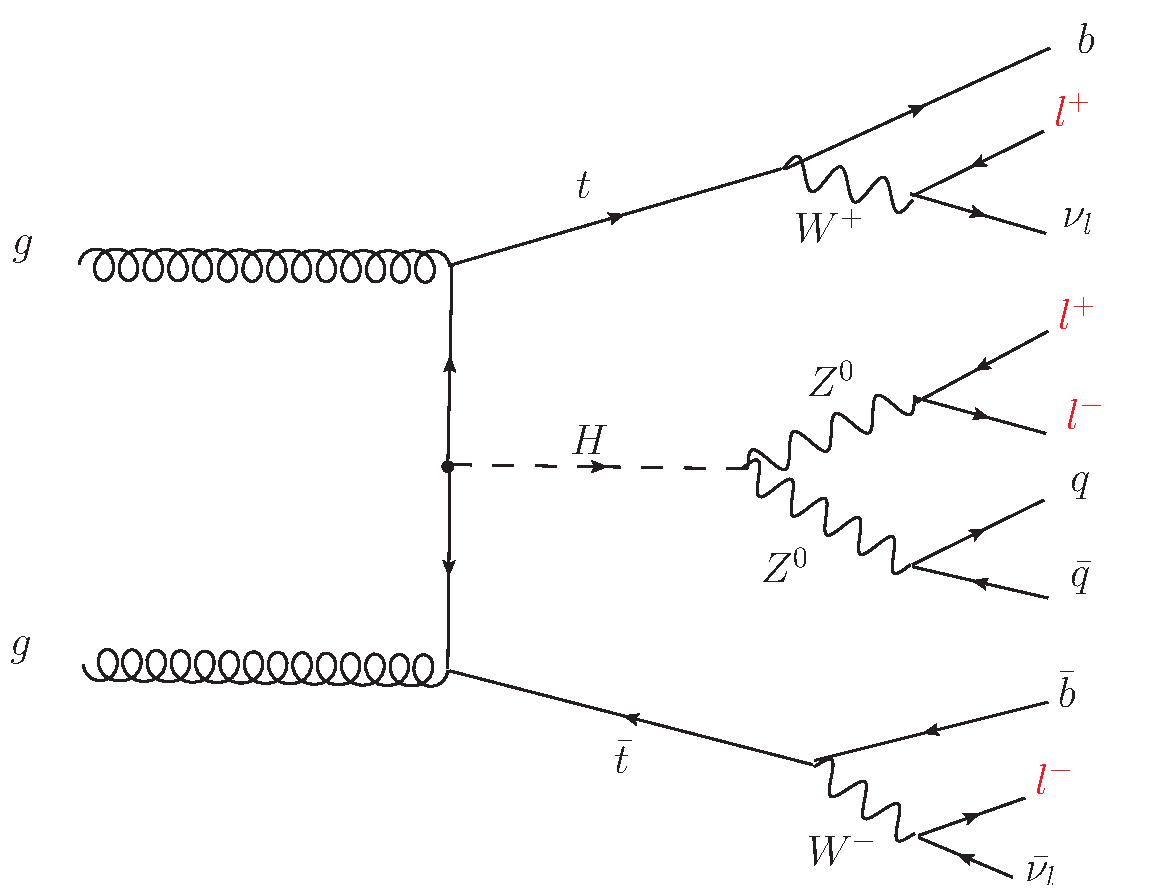
\includegraphics[width=0.30\textwidth]{figs/analysis/4l.pdf}} 
\end{tabular} 
\caption{Example feynman diagrams for the 3 \tth multi-lepton categories.}
\label{figure:theory_higgsdiagrams}
\end{figure}



Three Higgs boson decays are relevant for this analysis: \WW,
\twotau and \ZZ. The top and anti-top quarks decay  in
\Wb. Each \W boson decays either 
leptonically (l=$e^\pm$, $\mu^\pm$,$\tau^\pm$) with missing energy or hadronically. 
Table \ref{ana:table_decay} provides the fractional contribution of the main 
Higgs decay modes at the generator level to \tth search channels. These
numbers will be modified by lepton acceptances. 

\begin{table}[htbp]
  \begin{center} 
    \caption{Contributions of the main Higgs decay modes to the 3 multi-lepton
      \tth signatures at generation level.
      }\label{ana:table_decay} 
      \begin{tabular}{l|c|c|c} 
      \hline\hline
  Signature & $H \rightarrow WW$  & $H\rightarrow \tau\tau$  & $H \rightarrow
  ZZ$  \\\hline
  Same-sign &  $100\%$ & -- & -- \\
  3 leptons  &  $71\%$ & $20\%$ & $9\%$ \\
  4 leptons  &  $53\%$ & $30\%$ & $17\%$  \\
     \hline
    \end{tabular}
  \end{center}
\end{table}


All modes are generally dominated by the $WW$ signature, though the 3$\ell$ and 4$\ell$
channels possess some contribution from the$\tau\tau$ and $ZZ$ decays. 


The signal is expected to be characterized by the presence of 2 b-quark jets from
the top quark decays, leptons from vector boson and tau decays,
a high jet multiplicity, and missing energy. In general, the number of leptons is anti-correlated 
with the number of jets, since a vector boson can either decay leptonically 
or hadronically. For \hww, the light quark multiplicity, $N_q$, and the
number of leptons, $N_l$, follow this relation: $2N_l+N_q+N_b=10$.

\begin{itemize}
\item In the same-sign channel, the \tth final state contains 6 quarks. These events
are then characterized by a large jet multiplicity.

\item In the 3 lepton channel, the \tth final state contains 4 quarks from the hard scatter.

\item In the 4 lepton channel, the \tth final state contains a small number of light
quarks, 0 (\hww case), 2 or 4 (\hzz case).


\end{itemize} 

\section{Background Overview}

Background processes can be sorted into two categories:

\begin{itemize}

\item Events with a non prompt or a fake lepton selected as prompt
  lepton. These processes cannot lead to a final state compatible with the
  signal signature without a mis-reconstructed object. This category includes
  events with a prompt lepton but with mis-reconstructed charge\footnote{Charge mis-identification is almost exclusively a phenomenon of electrons at our energy scales. While it is
  is possible for both electrons and muons to have an extremely straight track, whose direction of curvature is difficult to measure, the happens only at extremely high momentum. 
  Electrons on the other hand may interact with the detector material, resulting in bremsstrahlung. The bremsstrahlung photon may subsequently convert resulting in 2 additional
  tracks near the original electron. This process, called a trident process, may cause a mismatching of the electron cluster with the original electron track and thus
  a charge-mis identification and happens also at low energies}and events
  with jets that "fake" leptons.  These processes are rejected with tight object isolation and identification criteria, requiring a large jet multiplicity, and veto-ing events
  consistent with a leptonically decaying Z boson. 

  The main backgrounds of this sort are: \ttbar and \zj.
  Data-driven techniques are used to control some of these processes.
  Their importance varies depending on the channel.

\item Events which can lead to the same final state as the signal (irreducible
  backgrounds).
 The main background of this category are: \ttV, \WZ, and \ZZ.
 They are modeled using the Monte Carlo simulations. In general,
 these backgrounds are combatted with jet and b-tagged jet requirements. 
 Although the jet multiplicity of \ttV is high, the multiplicity of \tth 
 events is still higher. 

\end{itemize}


\section{Analysis Strategy} 


ADD SOMETHING HERE FOR HOW TO CALCULATE A CROSS-SECTION

The analysis search is conducted in 3 channels, based on counting of fully identified
leptons: 2 SS leptons, 3 leptons,and 4 leptons. The lepton counting occurs before additional object cuts are made in each individual 
channel to ensure orthogonality . The division into lepton channels rather than channels targeting specific decay modes
allows channels with different sensitivities to considered separately. We further divide the 2$\ell$ SS into sub channels
based on the number of jets and flavor of the leptons and the 4$\ell$ channel into sub-channels enriched and depleted in OS leptons arising from Z decays. 

The channels are fed into a Poisson model 



